% \documentclass[ba,preprint]{imsart}% use this for supplement article
\documentclass[ba]{imsart}
%
\pubyear{2021}
\volume{TBA}
\issue{TBA}
% \doi{0000}
\arxiv{2010.00000}
\firstpage{1}
\lastpage{1}

%
\usepackage{amsthm}
\usepackage{amsmath}
\usepackage{natbib}
\usepackage[colorlinks,citecolor=blue,urlcolor=blue,filecolor=blue,backref=page]{hyperref}
\usepackage{graphicx}

\startlocaldefs
\numberwithin{equation}{section}
\theoremstyle{plain}
\newtheorem{thm}{Theorem}[section]
\endlocaldefs

\begin{document}

\begin{frontmatter}
\title{A Sample Document\support{Support information of the article.}}
\runtitle{A Sample Document}

\begin{aug}
\author{\fnms{First} \snm{Author}\thanksref{addr1,t1,t2,m1}\ead[label=e1]{first@somewhere.com}},
\author{\fnms{Second} \snm{Author}\thanksref{addr1,t3,m1,m2}\ead[label=e2]{second@somewhere.com}}
\and
\author{\fnms{Third} \snm{Author}\thanksref{addr2,t1,m2}%
\ead[label=e3]{third@somewhere.com}%
\ead[label=u1,url]{http://www.foo.com}}

\runauthor{F. Author et al.}

\address[addr1]{Address of the First and Second authors
     Usually a few lines long 
    \printead{e1} % print email address of "e1"
    \printead*{e2}
}

\address[addr2]{Address of the Third author
    Usually a few lines long
    Usually a few lines long
    \printead{e3}
    \printead{u1}
}

\thankstext{t1}{Some comment}
\thankstext{t2}{First supporter of the project}
\thankstext{t3}{Second supporter of the project}

\end{aug}

\begin{abstract}
The abstract should summarize the contents of the paper. It 
should be clear, descriptive, self-explanatory and not longer
than 200 words. It should also be suitable for publication in
abstracting services. Please avoid using math formulas as 
much as possible.

This is a sample input file.  Comparing it with the output it
generates can show you how to produce a simple document 
of your own.
\end{abstract}

\begin{keyword}[class=MSC]
\kwd[Primary ]{60K35}
\kwd{60K35}
\kwd[; secondary ]{60K35}
\end{keyword}

\begin{keyword}
\kwd{sample}
\kwd{\LaTeXe}
\end{keyword}

\end{frontmatter}

\section{Ordinary text}

The ends of words and sentences are marked by spaces. It doesn't
matter how many spaces you type; one is as good as 100.  The end of a
line counts as a space.

One or more blank lines denote the end of a paragraph.

Since any number of consecutive spaces are treated like a single one,
the formatting of the input file makes no difference to
\TeX, % The \TeX command generates the TeX logo.
but it makes a difference to you.  When you use
\LaTeX, % The \LaTeX command generates the LaTeX logo.
making your input file as easy to read as possible will be a great
help as you write your document and when you change it.  This sample
file shows how you can add comments to your own input file.

Because printing is different from typewriting, there are a number of
things that you have to do differently when preparing an input file
than if you were just typing the document directly.  Quotation marks
like ``this'' have to be handled specially, as do quotes within
quotes: ``\,`this' % \, separates the double and single quote.
is what I just wrote, not `that.'\,''

Dashes come in three sizes: a hyphen, %an intra-word dash,
a medium dash for number ranges like 1--2, and a punctuation dash in
place of a comma, semicolon, colon or parentheses ---like this.

A sentence-ending space should be larger than the space between words
within a sentence.  You sometimes have to type special commands in
conjunction with punctuation characters to get this right, as in the
following sentence.  Gnats, gnus,
etc.\ % `\ ' makes an inter-word space.
all begin with G\@.  % \@ marks end-of-sentence punctuation.
You should check the spaces after periods when reading your output to
make sure you haven't forgotten any special cases.  Generating an
ellipsis \ldots\ % `\ ' needed because TeX ignores spaces after
          % command names like \ldots made from \ + letters.
          %
          % Note how a `%' character causes TeX to ignore the
          % end of the input line, so these blank lines do not
          % start a new paragraph.
with the right spacing around the periods
requires a special  command.

\TeX\ interprets some common characters as commands, so you must type
special commands to generate them.  These characters include the
following:
%       \$ - arXiv do not like it...
        \& \% \# \{ and~\}.

In printing, text is emphasized by using an {\em
          italic\/} % The \/ command produces the tiny extra space that
               % should be added between a slanted and a following
               % unslanted letter.
type style.

\begin{em}
  A long segment of text can also be emphasized in this way.  Text
  within such a segment given additional emphasis with\/ {\em Roman}
  type.  Italic type loses its ability to emphasize and become simply
  distracting when used excessively.
\end{em}

It is sometimes necessary to prevent \TeX\ from breaking a line where
it might otherwise do so.  This may be at a space, as between the
``Mr.'' and ``Jones'' in
``Mr.~Jones'', % ~ produces an unbreakable interword space.
or within a word---especially when the word is a symbol like \mbox{\em
  itemnum\/} that makes little sense when hyphenated across lines.

\TeX\ is good at typesetting mathematical formulas like \( x-3y = 7 \)
or \( a_{1} > x^{2n} / y^{2n} > x' \).  Remember that a letter like
$x$ % $ ... $ and \( ... \) are equivalent
is a formula when it denotes a mathematical symbol, and should be
treated as one.


\section{Notes}

Footnotes\footnote{This is an example of a footnote.}  pose no
problem\footnote{And another one}.

\section{Displayed text}

Text is displayed by indenting it from the left margin.  Quotations
are commonly displayed.  There are short quotations
\begin{quote}
  This is a short a quotation.  It consists of a single paragraph of
  text.  There is no paragraph indentation.
\end{quote}
and longer ones.
\begin{quotation}
  This is a longer quotation.  It consists of two paragraphs of text.
  The beginning of each paragraph is indicated by an extra
  indentation.

  This is the second paragraph of the quotation.  It is just as dull
  as the first paragraph.
\end{quotation}
Another frequently displayed structure is a list.  The following is an
example of an {\em itemized} list, four levels deep.
\begin{itemize}
\item This is the first item of an itemized list.  Each item in the
  list is marked with a ``tick.''  The document style determines what
  kind of tick mark is used.
\item This is the second item of the list.  It contains another list
  nested inside it.  The three inner lists are an {\em itemized} list.
    \begin{itemize}
    \item This is the first item of an enumerated list that is nested
      within the itemized list.
    \item This is the second item of the inner list.  \LaTeX\ allows
      you to nest lists deeper than you really should.
    \end{itemize}
    This is the rest of the second item of the outer list.  It is no
    more interesting than any other part of the item.
   \item  This is the third item of the list.
\end{itemize}


The following is an example of an {\em enumerated} list, four levels
deep.
\begin{enumerate}
\item This is the first item of an enumerated list.  Each item in the
  list is marked with a ``tick.''  The document style determines what
  kind of tick mark is used.
\item This is the second item of the list.  It contains another list
  nested inside it.  The three inner lists are an {\em enumerated}
  list.
  \begin{enumerate}
  \item This is the first item of an enumerated list that is nested
    within the enumerated list.
  \item This is the second item of the inner list.  \LaTeX\ allows you
    to nest lists deeper than you really should.
  \end{enumerate}
  This is the rest of the second item of the outer list.  It is no
  more interesting than any other part of the item.
\item This is the third item of the list.
\end{enumerate}


The following is an example of a {\em description} list.
\begin{description}
\item[Cow] Highly intelligent animal that can produce milk out of grass.
\item[Horse] Less intelligent animal renowned for its legs.
\item[Human being] Not so intelligent animal convinced it can think.
\end{description}

You can even display poetry.
\begin{verse}
  There is an environment for verse
  \\ % The \\ command separates lines
  Whose features some poets will curse.  % within a stanza.

               % One or more blank lines separate stanzas.

  For instead of making\\
  Them do {\em all\/} line breaking, \\
  It allows them to put too many words on a line when they'd rather be
  forced to be terse.
\end{verse}

Mathematical formulas may also be displayed.  A displayed formula is
one-line long:

   \[  x' + y^{2} = z_{i}^{2};\]

   multiline formulas require special formatting instructions.

   Do not start a paragraph with a displayed equation, nor make one a
   paragraph by itself.

Example of a theorem:


\begin{thm}
All conjectures are interesting, but some conjectures are more
interesting than others.
\end{thm}

\begin{proof}
Obvious.
\end{proof}

\section{Tables and figures}
Cross reference to labeled table: As you can see in Table~\ref{sphericcase} on
page~\pageref{sphericcase} and also in Table~\ref{parset} on page~\pageref{parset}.


\begin{table*}
\begin{tabular}{crrrrc}
\hline
Equil. \\
Points & \multicolumn{1}{c}{$x$} & \multicolumn{1}{c}{$y$} & \multicolumn{1}{c}{$z$} & \multicolumn{1}{c}{$C$} &
S \\
\hline
$~~L_1$ & $-$2.485252241 & 0.000000000 & 0.017100631 & 8.230711648 & U \\
$~~L_2$ &    0.000000000 & 0.000000000 & 3.068883732 & 0.000000000 & S \\
$~~L_3$ &    0.009869059 & 0.000000000 & 4.756386544 & $-$0.000057922 & U \\
$~~L_4$ &    0.210589855 & 0.000000000 & $-$0.007021459 & 9.440510897 & U \\
$~~L_5$ &    0.455926604 & 0.000000000 & $-$0.212446624 & 7.586126667 & U \\
$~~L_6$ &    0.667031314 & 0.000000000 & 0.529879957 & 3.497660052 & U \\
$~~L_7$ &    2.164386674 & 0.000000000 & $-$0.169308438 & 6.866562449 & U \\
$~~L_8$ &    0.560414471 & 0.421735658 & $-$0.093667445 & 9.241525367 & U \\
$~~L_9$ &    0.560414471 & $-$0.421735658 & $-$0.093667445 & 9.241525367 & U
\\
$~~L_{10}$ & 1.472523232 & 1.393484549 & $-$0.083801333 & 6.733436505 & U \\
$~~L_{11}$ & 1.472523232 & $-$1.393484549 & $-$0.083801333 & 6.733436505 & U
\\ \hline
\end{tabular}
\caption{The spherical case ($I_1=0$, $I_2=0$)}
\label{sphericcase}
\end{table*}


A major point of difference lies in the value of the specific
production rate $\pi$ for large values of the specific growth rate
$\mu$.  Already in the early publications \cite{akaike,dyke,greene} it
appeared that high glucose concentrations in the production phase are
well correlated with a low penicillin yield (the ``glucose
effect''). It has been confirmed recently
\cite{akaike,dyke,greene,hilbe} that high glucose concentrations
inhibit the synthesis of the enzymes of the penicillin pathway, but
not the actual penicillin biosynthesis.  In other words, glucose
represses (and not inhibits) the penicillin biosynthesis.

These findings do not contradict the results of \cite{akaike} and of
\cite{hilbe} which were obtained for continuous culture fermentations.
Because for high values of the specific growth rate $\mu$ it is most
likely (as shall be discussed below) that maintenance metabolism
occurs, it can be shown that in steady state continuous culture
conditions, and with $\mu$ described by a Monod kinetics
\begin{equation}
    C_{s}  =  K_{M} \frac{\mu/\mu_{x}}{1-\mu/\mu_{x}} \label{cs}
\end{equation}
Pirt \& Rhigelato determined $\pi$ for $\mu$ between
$0.023$ and $0.086$ h$^{-1}$.
They also reported a value $\mu_{x} \approx 0.095$
h$^{-1}$, so that for their experiments $\mu/\mu_{x}$ is in the range
of $0.24$ to $0.9$.
Substituting $K _M$ in equation (\ref{cs}) by
the value $K_{M}=1$ g/L as used by \cite{akaike}, one finds
with the above equation $0.3 < C_{s} < 9$ g/L. This agrees with
the work of  \cite{hilbe}, who reported that penicillin biosynthesis
repression only occurs at glucose concentrations from $C_{s}=10$ g/L on.
The conclusion is that the glucose concentrations in the experiments of
Pirt \& Rhigelato probably were too low for glucose repression to be
detected. The experimental data published by Ryu \& Hospodka
are not detailed sufficiently to permit a similar analysis.


\begin{table}
\begin{tabular}{lrll}
\hline
\multicolumn{2}{l}{\it parameter} & {\it Set 1} & {\it Set 2}\\
\hline
$\mu_{x}$           & [h$^{-1}$]  & 0.092       & 0.11          \\
$K_{x}$             & [g/g DM]     & 0.15        & 0.006         \\
$\mu_{p}$           & [g/g DM h]  & 0.005       & 0.004         \\
$K_{p}$             & [g/L]        & 0.0002      & 0.0001        \\
$K_{i}$             & [g/L]        & 0.1         & 0.1           \\
$Y_{x/s}$           & [g DM/g]     & 0.45        & 0.47          \\
$Y_{p/s}$           & [g/g]        & 0.9         & 1.2           \\
$k_{h}$             & [h$^{-1}$]  & 0.04        & 0.01          \\
$m_{s}$             & [g/g DM h]  & 0.014       & 0.029         \\
\hline
\end{tabular}
\caption{Parameter sets used by Bajpai \& Reu\ss\ }\label{parset}
\end{table}


Bajpai \& Reu\ss\ decided to disregard the differences between time
constants for the two regulation mechanisms (glucose repression or
inhibition) because of the relatively very long fermentation times,
and therefore proposed a Haldane expression for $\pi$.

It is interesting that simulations with the \cite{hilbe} model for the
initial conditions given by these authors indicate that, when the
remaining substrate is fed at a constant rate, a considerable and
unrealistic amount of penicillin is produced when the glucose
concentration is still very high \cite{dyke,greene,hilbe} Simulations
with the Bajpai \& Reu\ss\ model correctly predict almost no
penicillin production in similar conditions.

% figure 1
\begin{figure} 
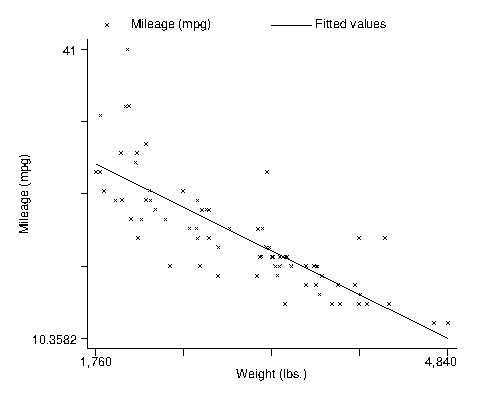
\includegraphics{fig001}
\caption[]{Pathway of the penicillin G biosynthesis.}
\label{penG}
\end{figure}

Sample of cross-reference to figure.
Figure~\ref{penG} shows that is not easy to get something on paper.



\section{Headings}

\subsection{Subsection}

Carr--Goldstein based their model on balancing methods and biochemical
know\-ledge. The original model (1980) contained an equation for the
oxygen dynamics which has been omitted in a second paper (1981). This
simplified model shall be discussed here.

\subsubsection{Subsubsection}

Carr--Goldstein based their model on balancing methods and biochemical
know\-ledge. The original model (1980) contained an equation for the
oxygen dynamics which has been omitted in a second paper (1981). This
simplified model shall be discussed here.

\section{Equations and the like}

Two equations:
\begin{equation}
    C_{s}  =  K_{M} \frac{\mu/\mu_{x}}{1-\mu/\mu_{x}} \label{ccs}
\end{equation}
and
\begin{equation}
    G = \frac{P_{\rm opt} - P_{\rm ref}}{P_{\rm ref}} \mbox{\ }100 \mbox{\ }(\%).
\end{equation}

Two equation arrays:

\begin{eqnarray}
  \frac{dS}{dt} & = & - \sigma X + s_{F} F\\
  \frac{dX}{dt} & = &   \mu    X\\
  \frac{dP}{dt} & = &   \pi    X - k_{h} P\\
  \frac{dV}{dt} & = &   F
\end{eqnarray}
and
\begin{eqnarray}
 \mu_{\rm substr} & = & \mu_{x} \frac{C_{s}}{K_{x}C_{x}+C_{s}}  \\
 \mu              & = & \mu_{\rm substr} - Y_{x/s}(1-H(C_{s}))(m_{s}+\pi /Y_{p/s}) \\
 \sigma           & = & \mu_{\rm substr}/Y_{x/s}+ H(C_{s}) (m_{s}+ \pi /Y_{p/s}).
\end{eqnarray}


%%%%%%%%%%%%%%%%%%%%%%%%%%%%%%%%%%%%%%%%%%%%%%
%% Supplementary Material, if any, should   %%
%% be provided in {supplement} environment  %%
%% with title and short description.        %%
%%%%%%%%%%%%%%%%%%%%%%%%%%%%%%%%%%%%%%%%%%%%%%
\begin{supplement}
\stitle{Title of Supplement A}
\sdescription{Short description of Supplement A.}
\end{supplement}
\begin{supplement}
\stitle{Title of Supplement B}
\sdescription{Short description of Supplement B.}
\end{supplement}

The following are some other citations to check that the bibliographc style
file is working correctly: \citet{akaike}, \citet*{akivarsq}, \citet{dyke},
\citet{greene}, \citet*{kstuart}, \citet{hilbetech}, \citet{hilbe},
\citet{hilbeglm}, \citet{maddalacntrsq}, and \citet*{companion}.  


\bibliographystyle{ba}
\bibliography{sample}

\begin{acks}[Acknowledgments]
And this is an acknowledgements section with a heading that was produced by the
$\backslash$section* command. Thank you all for helping me writing this
\LaTeX\ sample file.
\end{acks}


\end{document}

